%%%%%%%%%%%%%%%%%%%%%%%%%%%%%%%%%%%%%%%%%%%%%%%%%%%%%%%%%%%%%%%%%%%%%%
%         FILE:  main.tex
%
%        USAGE:  ---
%
%  DESCRIPTION:  Presentation for MathSem Seminar QM
%
%      OPTIONS:  see different input's below
% REQUIREMENTS:  full LaTeX installations
%         BUGS:  ---
%        NOTES:  ---
%       AUTHOR:  Pascal Stump, pascal-stump@bluewin.ch
%      VERSION:  ---
%      CREATED:  26.Apr.2014
%     REVISION:  ---
%%%%%%%%%%%%%%%%%%%%%%%%%%%%%%%%%%%%%%%%%%%%%%%%%%%%%%%%%%%%%%%%%%%%%%

%%% LaTeX PREAMBLE
\documentclass[compressd]
{beamer}
\usecolortheme[named=orange]{structure}
\mode<presentation>
{
	\usetheme{Frankfurt}
}

\setbeamertemplate{itemize items}[default]
\setbeamertemplate{enumerate items}[default]

%%%%%%%%%%%%%%%%%%%%%%%%%%%%%%%%%%%%%%%%%%%%%%%%%%%%%%%%%%%%%%%%%%%%%%
%         FILE:  normalHeader.tex
%
%        USAGE:  ---
%
%  DESCRIPTION:  normal header for LaTeX files
%
%      OPTIONS:  ---
% REQUIREMENTS:  full LaTeX installations
%                main document
%                biber for bibliography
%         BUGS:  
%        NOTES:  ---
%       AUTHOR:  Pascal Stump, pascal-stump@bluewin.ch
%      VERSION:  see git repo
%      CREATED:  18.Apr.2014 - 17:50
%     REVISION:  see git repo
%%%%%%%%%%%%%%%%%%%%%%%%%%%%%%%%%%%%%%%%%%%%%%%%%%%%%%%%%%%%%%%%%%%%%%

%%% language definitions
\usepackage[T1]{fontenc}         % Umlaute as one character
\usepackage[utf8]{inputenc}      % character encoding

\usepackage[main=ngerman,        % main language in document
            english,             % other languages
            ngerman]
           {babel}               % correct language support
                                 %   change language within document :
                                 %     \selectlanguage{}

\usepackage[babel,               % use babel in background
            german=swiss]        % define german's style, also:
                                 %   quotes; guillemets; swiss
           {csquotes}            % quotes standardisation for whole
                                 %   document, usage: \enquote{}
                                 %   csquotes does not now
                                 %   nswissgerman, therefor definition:
\DeclareQuoteAlias{german}{nswissgerman}
                                 %   definition below only works with
                                 %     babel=german
\defineshorthand{"`}{\openautoquote}
\defineshorthand{"'}{\closeautoquote}

%%% miscellaneous
\usepackage{hyperref}            % url, clickable pdf

\usepackage[style=ieee,
            backend=biber,
            language=auto]
            {biblatex}           % citing of references
                                 %   usage:
                                 %     \bibliography{pathTo}
                                 %     \cite[prenote][postnote]{key}
                                 %     \printbibliography
\DeclareLanguageMapping{nswissgerman}{ngerman}

\usepackage{lipsum}              % lorem ipsum text include
                                 %   \lipsum
                                 %   \lipsum[4-6]
                                 
%%% tabularx
\usepackage{tabularx}

%%% caption
\usepackage[font=small]{caption}
% ähndern der Schriftgrösse bei caption


%%% preview
%\usepackage[showlables,sections,floats,textmath,displaymath]{preview}

%%% picture & graphics
\usepackage{tikz}                % TikZ graphics
\usetikzlibrary{arrows,        % include into main only what needed
%                 decorations,
%                 pathmorphing,
%                 backgrounds,
%                 positioning,
%                 fit,
%                 petri,
%                 calc,
%                 intersections,
%                 through
                shapes}

%%% units
\usepackage{siunitx}             % SI unit  \si{unit} or \SI{value}{unit}
\sisetup{per-mode=symbol-or-fraction,
         detect-shape,
         range-phrase = { \translate{bis} } }
                                 %   fraction; font shape auto detect

%%% chemistry
\usepackage[version=3]{mhchem}   % easy typesetting of chemical
                                 %   formula, usage:
                                 %     \ce{1/2H20}
                                 %     \ce{^{227}_{90}Th+}

\usepackage{chemfig}             % drawing molecules (with TikZ)
                                 %   usage:
                                 %     \chemfig{}
% http://mirror.switch.ch/ftp/mirror/tex/macros/generic/chemfig/chemfig_doc_en.pdf

%%% electronic                   % drawing electrical circuits (with
\usepackage[europeanvoltages,
            europeancurrents,
            europeanresistors,   % rectangular shape
            americaninductors,   % "4-bumbs" shape
            europeanports,       % rectangular logic ports
            siunitx,             % #1<#2>
            emptydiodes,
            noarrowmos,
            smartlabels]         % lables are rotated in a smart way
           {circuitikz}          %   TikZ), usage:
                                 %   \begin{circuitikz}
% http://mirror.switch.ch/ftp/mirror/tex/graphics/pgf/contrib/circuitikz/circuitikzmanual.pdf



%%% other packages
\usepackage{standalone}

%%% BibTeX document
%\bibliography{testTex/testBibtex}

%%% Title
\title[MathSem QM]{Mathematisches Seminar Quantenmechanik}
\subtitle{Atomuhr}
\author{Stefan Steiner \and Pascal Stump}
\institute{HSR Hochschule für Technik Rapperswil}
\date{04.\,Mai 2014}


%%%%%%%%%%%%%%%%%%%%%%%%%%%%%%%%%%%%%%%%%%%%%%%%%%%%%%%%%%%%%%%%%%%%%%
%%% BEGIN DOCUMENT
\begin{document}
	
	%%% input tex files
	\begin{frame}
		\titlepage
	\end{frame}
	
	%%%
	% 00_Themen; Begrüssung
	\section*{Begrüssung}
	% 00_themen

%\subsection*[Themen]{Themen}
\begin{frame}
\tableofcontents
\end{frame}





%%% Local Variables: 
%%% mode: latex
%%% TeX-master: "../main"
%%% End: 

	
	% 01_Einleitung
	\section{Einleitung}
	% 01_einleitung

%% Periodic Table addapted from http://www.texample.net/tikz/examples/periodic-table-of-chemical-elements/

\newcommand{\CommonElementTextFormat}[4]
{
  \begin{minipage}{2.2cm}
    \centering
      {\textbf{#1} \hfill #2}%
      \linebreak \linebreak
      {\textbf{#3}}%
      \linebreak \linebreak
      {{#4}}
  \end{minipage}
}

\newcommand{\NaturalElementTextFormat}[4]
{
  \CommonElementTextFormat{#1}{#2}{\Huge {#3}}{#4}
}

% \newcommand{\OutlineText}[1]
% {
%   % Couldn't find a nicer way of doing an outline font with TikZ
%   % other than using pdfliteral 1 Tr
%   %
%   \pdfliteral direct {0.5 w 1 Tr}{#1}%
%   \pdfliteral direct {1 w 0 Tr}%
% }

\newcommand{\SyntheticElementTextFormat}[4]
{
%  \CommonElementTextFormat{#1}{#2}{\OutlineText{\LARGE #3}}{#4}
  \CommonElementTextFormat{#1}{#2}{\Huge #3}{#4}
}



\subsection{Vergleich Atomuhren}

\begin{frame}
  \frametitle{Vergleich Verschiedener Atomuhren}

  \begin{columns}
    \column{.5\textwidth}
    \begin{description}
    \item[1949] Ammoniak
    \item[1967] \num{9192631770} Caesium-133
    \item[1998] Frequenzkamm
    \item[2014] \num{e-18}
    \end{description}

    \column{.5\textwidth}
    \begin{tabularx}{\columnwidth}{X r r}
      Quarz         & & \num{e-5}\\
      OCXO          & \SI{10}{\mega\hertz}    & \num{2e-8}\\
      \ce{NH3}      & \SI{23.79}{\giga\hertz} & \num{2e-8}\\
      \ce{^{87}Ru}  & \SI{6.83}{\giga\hertz}  & \num{e-9}\\
      \ce{^{133}Cs} & \SI{9.19}{\giga\hertz}  & \num{e-15}\\
      \ce{^{1}H}    & \SI{1.42}{\giga\hertz}  & \num{5e-16}
    \end{tabularx}
  \end{columns}

\end{frame}

\begin{frame}
  \frametitle{Verwendete Elemente}

\begin{figure}
\centering
\begin{tikzpicture}[font=\sffamily, scale=0.21, transform shape]

%% Fill Color Styles
  \tikzstyle{ElementFill} = [fill=yellow!15]
  \tikzstyle{AlkaliMetalFill} = [fill=blue!55]
  \tikzstyle{AlkalineEarthMetalFill} = [fill=blue!40]
  \tikzstyle{MetalFill} = [fill=blue!25]
  \tikzstyle{MetalloidFill} = [fill=orange!25]
  \tikzstyle{NonmetalFill} = [fill=green!25]
  \tikzstyle{HalogenFill} = [fill=green!40]
  \tikzstyle{NobleGasFill} = [fill=green!55]
  \tikzstyle{LanthanideActinideFill} = [fill=purple!25]
  \tikzstyle{AtomicClockElecFill} = [fill=yellow!75]
  \tikzstyle{AtomicClockOpticFill} = [fill=red!75]

%% Element Styles
  \tikzstyle{Element} = [draw=black, ElementFill,
    minimum width=2.75cm, minimum height=2.75cm, node distance=2.75cm]
  \tikzstyle{AlkaliMetal} = [Element, AlkaliMetalFill]
  \tikzstyle{AlkalineEarthMetal} = [Element, AlkalineEarthMetalFill]
  \tikzstyle{Metal} = [Element, MetalFill]
  \tikzstyle{Metalloid} = [Element, MetalloidFill]
  \tikzstyle{Nonmetal} = [Element, NonmetalFill]
  \tikzstyle{Halogen} = [Element, HalogenFill]
  \tikzstyle{NobleGas} = [Element, NobleGasFill]
  \tikzstyle{LanthanideActinide} = [Element, LanthanideActinideFill]
  \tikzstyle{AtomicClockElec} = [Element, AtomicClockElecFill]
  \tikzstyle{AtomicClockOptic} = [Element, AtomicClockOpticFill]
  \tikzstyle{PeriodLabel} = [font={\sffamily\LARGE}, node distance=2.0cm]
  \tikzstyle{GroupLabel} = [font={\sffamily\LARGE}, minimum width=2.75cm, node distance=2.0cm]
  \tikzstyle{TitleLabel} = [font={\sffamily\Huge\bfseries}]

%% Group 1 - IA
  \only<1>{  \node[name=H, Element] {\NaturalElementTextFormat{1}{1.0079}{H}{Hydrogen}};}
  \only<2->{  \node[name=H, AtomicClockElec] {\NaturalElementTextFormat{1}{1.0079}{H}{Hydrogen}};}
  \node[name=Li, below of=H, AlkaliMetal] {\NaturalElementTextFormat{3}{6.941}{Li}{Lithium}};
  \node[name=Na, below of=Li, AlkaliMetal] {\NaturalElementTextFormat{11}{22.990}{Na}{Sodium}};
  \node[name=K, below of=Na, AlkaliMetal] {\NaturalElementTextFormat{19}{39.098}{K}{Potassium}};
  \only<1>{  \node[name=Rb, below of=K, AlkaliMetal] {\NaturalElementTextFormat{37}{85.468}{Rb}{Rubidium}};}
  \only<2->{  \node[name=Rb, below of=K, AtomicClockElec] {\NaturalElementTextFormat{37}{85.468}{Rb}{Rubidium}};}
  \only<1>{  \node[name=Cs, below of=Rb, AlkaliMetal] {\NaturalElementTextFormat{55}{132.91}{Cs}{Caesium}};}
  \only<2->{  \node[name=Cs, below of=Rb, AtomicClockElec] {\NaturalElementTextFormat{55}{132.91}{Cs}{Caesium}};}
  \node[name=Fr, below of=Cs, AlkaliMetal] {\NaturalElementTextFormat{87}{223}{Fr}{Francium}};

%% Group 2 - IIA
  \only<-2>{  \node[name=Be, right of=Li, AlkalineEarthMetal] {\NaturalElementTextFormat{4}{9.0122}{Be}{Beryllium}};}
  \only<3->{  \node[name=Be, right of=Li, AtomicClockOptic] {\NaturalElementTextFormat{4}{9.0122}{Be}{Beryllium}};}
  \only<-2>{  \node[name=Mg, below of=Be, AlkalineEarthMetal] {\NaturalElementTextFormat{12}{24.305}{Mg}{Magnesium}};}
  \only<3->{  \node[name=Mg, below of=Be, AtomicClockOptic] {\NaturalElementTextFormat{12}{24.305}{Mg}{Magnesium}};}
  \only<-2>{  \node[name=Ca, below of=Mg, AlkalineEarthMetal] {\NaturalElementTextFormat{20}{40.078}{Ca}{Calcium}};}
  \only<3->{  \node[name=Ca, below of=Mg, AtomicClockOptic] {\NaturalElementTextFormat{20}{40.078}{Ca}{Calcium}};}
  \only<-2>{  \node[name=Sr, below of=Ca, AlkalineEarthMetal] {\NaturalElementTextFormat{38}{87.62}{Sr}{Strontium}};}
  \only<3->{  \node[name=Sr, below of=Ca, AtomicClockOptic] {\NaturalElementTextFormat{38}{87.62}{Sr}{Strontium}};}
  \node[name=Ba, below of=Sr, AlkalineEarthMetal] {\NaturalElementTextFormat{56}{137.33}{Ba}{Barium}};
  \node[name=Ra, below of=Ba, AlkalineEarthMetal] {\NaturalElementTextFormat{88}{226}{Ra}{Radium}};

%% Group 3 - IIIB
  \node[name=Sc, right of=Ca, Metal] {\NaturalElementTextFormat{21}{44.956}{Sc}{Scandium}};
  \node[name=Y, below of=Sc, Metal] {\NaturalElementTextFormat{39}{88.906}{Y}{Yttrium}};
  \node[name=LaLu, below of=Y, LanthanideActinide] {\NaturalElementTextFormat{57-71}{}{La-}{Lanthanide}};
  \node[name=AcLr, below of=LaLu, LanthanideActinide] {\NaturalElementTextFormat{89-103}{}{Ac-}{Actinide}};
  % \node[name=LaLu, below of=Y, LanthanideActinide] {\NaturalElementTextFormat{57-71}{}{La-Lu}{Lanthanide}};
  % \node[name=AcLr, below of=LaLu, LanthanideActinide] {\NaturalElementTextFormat{89-103}{}{Ac-Lr}{Actinide}};

%% Group 4 - IVB
  \node[name=Ti, right of=Sc, Metal] {\NaturalElementTextFormat{22}{47.867}{Ti}{Titanium}};
  \node[name=Zr, below of=Ti, Metal] {\NaturalElementTextFormat{40}{91.224}{Zr}{Zirconium}};
  \node[name=Hf, below of=Zr, Metal] {\NaturalElementTextFormat{72}{178.49}{Hf}{Halfnium}};
  \node[name=Rf, below of=Hf, Metal] {\SyntheticElementTextFormat{104}{261}{Rf}{Rutherfordium}};

%% Group 5 - VB
  \node[name=V, right of=Ti, Metal] {\NaturalElementTextFormat{23}{50.942}{V}{Vanadium}};
  \node[name=Nb, below of=V, Metal] {\NaturalElementTextFormat{41}{92.906}{Nb}{Niobium}};
  \node[name=Ta, below of=Nb, Metal] {\NaturalElementTextFormat{73}{180.95}{Ta}{Tantalum}};
  \node[name=Db, below of=Ta, Metal] {\SyntheticElementTextFormat{105}{262}{Db}{Dubnium}};

%% Group 6 - VIB
  \node[name=Cr, right of=V, Metal] {\NaturalElementTextFormat{24}{51.996}{Cr}{Chromium}};
  \node[name=Mo, below of=Cr, Metal] {\NaturalElementTextFormat{42}{95.94}{Mo}{Molybdenum}};
  \node[name=W, below of=Mo, Metal] {\NaturalElementTextFormat{74}{183.84}{W}{Tungsten}};
  \node[name=Sg, below of=W, Metal] {\SyntheticElementTextFormat{106}{266}{Sg}{Seaborgium}};

%% Group 7 - VIIB
  \node[name=Mn, right of=Cr, Metal] {\NaturalElementTextFormat{25}{54.938}{Mn}{Manganese}};
  \node[name=Tc, below of=Mn, Metal] {\NaturalElementTextFormat{43}{96}{Tc}{Technetium}};
  \node[name=Re, below of=Tc, Metal] {\NaturalElementTextFormat{75}{186.21}{Re}{Rhenium}};
  \node[name=Bh, below of=Re, Metal] {\SyntheticElementTextFormat{107}{264}{Bh}{Bohrium}};

%% Group 8 - VIIIB
  \node[name=Fe, right of=Mn, Metal] {\NaturalElementTextFormat{26}{55.845}{Fe}{Iron}};
  \node[name=Ru, below of=Fe, Metal] {\NaturalElementTextFormat{44}{101.07}{Ru}{Ruthenium}};
  \node[name=Os, below of=Ru, Metal] {\NaturalElementTextFormat{76}{190.23}{Os}{Osmium}};
  \node[name=Hs, below of=Os, Metal] {\SyntheticElementTextFormat{108}{277}{Hs}{Hassium}};

%% Group 9 - VIIIB
  \node[name=Co, right of=Fe, Metal] {\NaturalElementTextFormat{27}{58.933}{Co}{Cobalt}};
  \node[name=Rh, below of=Co, Metal] {\NaturalElementTextFormat{45}{102.91}{Rh}{Rhodium}};
  \node[name=Ir, below of=Rh, Metal] {\NaturalElementTextFormat{77}{192.22}{Ir}{Iridium}};
  \node[name=Mt, below of=Ir, Metal] {\SyntheticElementTextFormat{109}{268}{Mt}{Meitnerium}};

%% Group 10 - VIIIB
  \node[name=Ni, right of=Co, Metal] {\NaturalElementTextFormat{28}{58.693}{Ni}{Nickel}};
  \node[name=Pd, below of=Ni, Metal] {\NaturalElementTextFormat{46}{106.42}{Pd}{Palladium}};
  \node[name=Pt, below of=Pd, Metal] {\NaturalElementTextFormat{78}{195.08}{Pt}{Platinum}};
  \node[name=Ds, below of=Pt, Metal] {\SyntheticElementTextFormat{110}{281}{Ds}{Darmstadtium}};

%% Group 11 - IB
  \node[name=Cu, right of=Ni, Metal] {\NaturalElementTextFormat{29}{63.546}{Cu}{Copper}};
  \node[name=Ag, below of=Cu, Metal] {\NaturalElementTextFormat{47}{107.87}{Ag}{Silver}};
  \node[name=Au, below of=Ag, Metal] {\NaturalElementTextFormat{79}{196.97}{Au}{Gold}};
  \node[name=Rg, below of=Au, Metal] {\SyntheticElementTextFormat{111}{280}{Rg}{Roentgenium}};

%% Group 12 - IIB
  \node[name=Zn, right of=Cu, Metal] {\NaturalElementTextFormat{30}{65.39}{Zn}{Zinc}};
  \node[name=Cd, below of=Zn, Metal] {\NaturalElementTextFormat{48}{112.41}{Cd}{Cadmium}};
  \only<-2>{  \node[name=Hg, below of=Cd, Metal] {\NaturalElementTextFormat{80}{200.59}{Hg}{Mercury}};}
  \only<3->{  \node[name=Hg, below of=Cd, AtomicClockOptic] {\NaturalElementTextFormat{80}{200.59}{Hg}{Mercury}};}
  \node[name=Uub, below of=Hg, Metal] {\SyntheticElementTextFormat{112}{285}{Uub}{Ununbium}};

%% Group 13 - IIIA
  \node[name=Ga, right of=Zn, Metal] {\NaturalElementTextFormat{31}{69.723}{Ga}{Gallium}};
  \only<-2>{  \node[name=Al, above of=Ga, Metal] {\NaturalElementTextFormat{13}{26.982}{Al}{Aluminium}};}
  \only<3->{  \node[name=Al, above of=Ga, AtomicClockOptic] {\NaturalElementTextFormat{13}{26.982}{Al}{Aluminium}};}
  \node[name=B, above of=Al, Metalloid] {\NaturalElementTextFormat{5}{10.811}{B}{Boron}};
  \only<-2>{  \node[name=In, below of=Ga, Metal] {\NaturalElementTextFormat{49}{114.82}{In}{Indium}};}
  \only<3->{  \node[name=In, below of=Ga, AtomicClockOptic] {\NaturalElementTextFormat{49}{114.82}{In}{Indium}};}
  \node[name=Tl, below of=In, Metal] {\NaturalElementTextFormat{81}{204.38}{Tl}{Thallium}};
  \node[name=Uut, below of=Tl, Metal] {\SyntheticElementTextFormat{113}{284}{Uut}{Ununtrium}};

%% Group 14 - IVA
  \node[name=C, right of=B, Nonmetal] {\NaturalElementTextFormat{6}{12.011}{C}{Carbon}};
  \node[name=Si, below of=C, Metalloid] {\NaturalElementTextFormat{14}{28.086}{Si}{Silicon}};
  \node[name=Ge, below of=Si, Metalloid] {\NaturalElementTextFormat{32}{72.64}{Ge}{Germanium}};
  \node[name=Sn, below of=Ge, Metal] {\NaturalElementTextFormat{50}{118.71}{Sn}{Tin}};
  \node[name=Pb, below of=Sn, Metal] {\NaturalElementTextFormat{82}{207.2}{Pb}{Lead}};
  \node[name=Uuq, below of=Pb, Metal] {\SyntheticElementTextFormat{114}{289}{Uuq}{Ununquadium}};

%% Group 15 - VA
  \node[name=N, right of=C, Nonmetal] {\NaturalElementTextFormat{7}{14.007}{N}{Nitrogen}};
  \node[name=P, below of=N, Nonmetal] {\NaturalElementTextFormat{15}{30.974}{P}{Phosphorus}};
  \node[name=As, below of=P, Metalloid] {\NaturalElementTextFormat{33}{74.922}{As}{Arsenic}};
  \node[name=Sb, below of=As, Metalloid] {\NaturalElementTextFormat{51}{121.76}{Sb}{Antimony}};
  \node[name=Bi, below of=Sb, Metal] {\NaturalElementTextFormat{83}{208.98}{Bi}{Bismuth}};
  \node[name=Uup, below of=Bi, Metal] {\SyntheticElementTextFormat{115}{288}{Uup}{Ununpentium}};

%% Group 16 - VIA
  \node[name=O, right of=N, Nonmetal] {\NaturalElementTextFormat{8}{15.999}{O}{Oxygen}};
  \node[name=S, below of=O, Nonmetal] {\NaturalElementTextFormat{16}{32.065}{S}{Sulphur}};
  \node[name=Se, below of=S, Nonmetal] {\NaturalElementTextFormat{34}{78.96}{Se}{Selenium}};
  \node[name=Te, below of=Se, Metalloid] {\NaturalElementTextFormat{52}{127.6}{Te}{Tellurium}};
  \node[name=Po, below of=Te, Metalloid] {\NaturalElementTextFormat{84}{209}{Po}{Polonium}};
  \node[name=Uuh, below of=Po, Metal] {\SyntheticElementTextFormat{116}{293}{Uuh}{Ununhexium}};

%% Group 17 - VIIA
  \node[name=F, right of=O, Halogen] {\NaturalElementTextFormat{9}{18.998}{F}{Flourine}};
  \node[name=Cl, below of=F, Halogen] {\NaturalElementTextFormat{17}{35.453}{Cl}{Chlorine}};
  \node[name=Br, below of=Cl, Halogen] {\NaturalElementTextFormat{35}{79.904}{Br}{Bromine}};
  \node[name=I, below of=Br, Halogen] {\NaturalElementTextFormat{53}{126.9}{I}{Iodine}};
  \node[name=At, below of=I, Halogen] {\NaturalElementTextFormat{85}{210}{At}{Astatine}};
  \node[name=Uus, below of=At, Element] {\SyntheticElementTextFormat{117}{292}{Uus}{Ununseptium}}; 

%% Group 18 - VIIIA
  \node[name=Ne, right of=F, NobleGas] {\NaturalElementTextFormat{10}{20.180}{Ne}{Neon}};
  \node[name=He, above of=Ne, NobleGas] {\NaturalElementTextFormat{2}{4.0025}{He}{Helium}};
  \node[name=Ar, below of=Ne, NobleGas] {\NaturalElementTextFormat{18}{39.948}{Ar}{Argon}};
  \node[name=Kr, below of=Ar, NobleGas] {\NaturalElementTextFormat{36}{83.8}{Kr}{Krypton}};
  \node[name=Xe, below of=Kr, NobleGas] {\NaturalElementTextFormat{54}{131.29}{Xe}{Xenon}};
  \node[name=Rn, below of=Xe, NobleGas] {\NaturalElementTextFormat{86}{222}{Rn}{Radon}};
  \node[name=Uuo, below of=Rn, Nonmetal] {\SyntheticElementTextFormat{118}{294}{Uuo}{Ununoctium}}; 

%% Period
  \node[name=Period1, left of=H, PeriodLabel] {1};
  \node[name=Period2, left of=Li, PeriodLabel] {2};
  \node[name=Period3, left of=Na, PeriodLabel] {3}; 
  \node[name=Period4, left of=K, PeriodLabel] {4}; 
  \node[name=Period5, left of=Rb, PeriodLabel] {5};
  \node[name=Period6, left of=Cs, PeriodLabel] {6};
  \node[name=Period7, left of=Fr, PeriodLabel] {7};

%% Group
  \node[name=Group1, above of=H, GroupLabel] {1 \hfill IA};
  \node[name=Group2, above of=Be, GroupLabel] {2 \hfill IIA};
  \node[name=Group3, above of=Sc, GroupLabel] {3 \hfill IIIA};
  \node[name=Group4, above of=Ti, GroupLabel] {4 \hfill IVB};
  \node[name=Group5, above of=V, GroupLabel] {5 \hfill VB};
  \node[name=Group6, above of=Cr, GroupLabel] {6 \hfill VIB};
  \node[name=Group7, above of=Mn, GroupLabel] {7 \hfill VIIB};
  \node[name=Group8, above of=Fe, GroupLabel] {8 \hfill VIIIB};
  \node[name=Group9, above of=Co, GroupLabel] {9 \hfill VIIIB};
  \node[name=Group10, above of=Ni, GroupLabel] {10 \hfill VIIIB};
  \node[name=Group11, above of=Cu, GroupLabel] {11 \hfill IB};
  \node[name=Group12, above of=Zn, GroupLabel] {12 \hfill IIB};
  \node[name=Group13, above of=B, GroupLabel] {13 \hfill IIIA};
  \node[name=Group14, above of=C, GroupLabel] {14 \hfill IVA};
  \node[name=Group15, above of=N, GroupLabel] {15 \hfill VA};
  \node[name=Group16, above of=O, GroupLabel] {16 \hfill VIA};
  \node[name=Group17, above of=F, GroupLabel] {17 \hfill VIIA};
  \node[name=Group18, above of=He, GroupLabel] {18 \hfill VIIIA};

%% Lanthanide
  \node[name=La, below of=Rf, LanthanideActinide, yshift=-1cm] {\NaturalElementTextFormat{57}{138.91}{La}{Lanthanum}};
  \node[name=Ce, right of=La, LanthanideActinide] {\NaturalElementTextFormat{58}{140.12}{Ce}{Cerium}};
  \node[name=Pr, right of=Ce, LanthanideActinide] {\NaturalElementTextFormat{59}{140.91}{Pr}{Praseodymium}};
  \node[name=Nd, right of=Pr, LanthanideActinide] {\NaturalElementTextFormat{60}{144.24}{Nd}{Neodymium}};
  \node[name=Pm, right of=Nd, LanthanideActinide] {\NaturalElementTextFormat{61}{145}{Pm}{Promethium}};
  \node[name=Sm, right of=Pm, LanthanideActinide] {\NaturalElementTextFormat{62}{150.36}{Sm}{Samarium}};
  \node[name=Eu, right of=Sm, LanthanideActinide] {\NaturalElementTextFormat{63}{151.96}{Eu}{Europium}};
  \node[name=Gd, right of=Eu, LanthanideActinide] {\NaturalElementTextFormat{64}{157.25}{Gd}{Gadolinium}};
  \node[name=Tb, right of=Gd, LanthanideActinide] {\NaturalElementTextFormat{65}{158.93}{Tb}{Terbium}};
  \node[name=Dy, right of=Tb, LanthanideActinide] {\NaturalElementTextFormat{66}{162.50}{Dy}{Dysprosium}};
  \node[name=Ho, right of=Dy, LanthanideActinide] {\NaturalElementTextFormat{67}{164.93}{Ho}{Holmium}};
  \node[name=Er, right of=Ho, LanthanideActinide] {\NaturalElementTextFormat{68}{167.26}{Er}{Erbium}};
  \node[name=Tm, right of=Er, LanthanideActinide] {\NaturalElementTextFormat{69}{168.93}{Tm}{Thulium}};
  \only<-2>{  \node[name=Yb, right of=Tm, LanthanideActinide] {\NaturalElementTextFormat{70}{173.04}{Yb}{Ytterbium}};}
  \only<3->{  \node[name=Yb, right of=Tm, AtomicClockOptic] {\NaturalElementTextFormat{70}{173.04}{Yb}{Ytterbium}};}
  \node[name=Lu, right of=Yb, LanthanideActinide] {\NaturalElementTextFormat{71}{174.97}{Lu}{Lutetium}};

%% Actinide
  \node[name=Ac, below of=La, LanthanideActinide, yshift=-1cm] {\NaturalElementTextFormat{89}{227}{Ac}{Actinium}};
  \node[name=Th, right of=Ac, LanthanideActinide] {\NaturalElementTextFormat{90}{232.04}{Th}{Thorium}};
  \node[name=Pa, right of=Th, LanthanideActinide] {\NaturalElementTextFormat{91}{231.04}{Pa}{Protactinium}};
  \node[name=U, right of=Pa, LanthanideActinide] {\NaturalElementTextFormat{92}{238.03}{U}{Uranium}};
  \node[name=Np, right of=U, LanthanideActinide] {\SyntheticElementTextFormat{93}{237}{Np}{Neptunium}};
  \node[name=Pu, right of=Np, LanthanideActinide] {\SyntheticElementTextFormat{94}{244}{Pu}{Plutonium}};
  \node[name=Am, right of=Pu, LanthanideActinide] {\SyntheticElementTextFormat{95}{243}{Am}{Americium}};
  \node[name=Cm, right of=Am, LanthanideActinide] {\SyntheticElementTextFormat{96}{247}{Cm}{Curium}};
  \node[name=Bk, right of=Cm, LanthanideActinide] {\SyntheticElementTextFormat{97}{247}{Bk}{Berkelium}};
  \node[name=Cf, right of=Bk, LanthanideActinide] {\SyntheticElementTextFormat{98}{251}{Cf}{Californium}};
  \node[name=Es, right of=Cf, LanthanideActinide] {\SyntheticElementTextFormat{99}{252}{Es}{Einsteinium}};
  \node[name=Fm, right of=Es, LanthanideActinide] {\SyntheticElementTextFormat{100}{257}{Fm}{Fermium}};
  \node[name=Md, right of=Fm, LanthanideActinide] {\SyntheticElementTextFormat{101}{258}{Md}{Mendelevium}};
  \node[name=No, right of=Md, LanthanideActinide] {\SyntheticElementTextFormat{102}{259}{No}{Nobelium}};
  \node[name=Lr, right of=No, LanthanideActinide] {\SyntheticElementTextFormat{103}{262}{Lr}{Lawrencium}};

%% Draw dotted lines connecting Lanthanide breakout to main table
  \draw (LaLu.north west) edge[dotted] (La.north west)
        (LaLu.north east) edge[dotted] (Lu.north east)
        (LaLu.south west) edge[dotted] (La.south west)
        (LaLu.south east) edge[dotted] (Lu.south east);
%% Draw dotted lines connecting Actinide breakout to main table
  \draw (AcLr.north west) edge[dotted] (Ac.north west)
        (AcLr.north east) edge[dotted] (Lr.north east)
        (AcLr.south west) edge[dotted] (Ac.south west)
        (AcLr.south east) edge[dotted] (Lr.south east);

% %% Legend
%   \draw[black, AlkaliMetalFill] ($(La.north -| Fr.west) + (1em,-0.0em)$)
%     rectangle +(1em, 1em) node[right, yshift=-1ex]{Alkali Metal};
%   \draw[black, AlkalineEarthMetalFill] ($(La.north -| Fr.west) + (1em,-1.5em)$)
%     rectangle +(1em, 1em) node[right, yshift=-1ex]{Alkaline Earth Metal};
%   \draw[black, MetalFill] ($(La.north -| Fr.west) + (1em,-3.0em)$)
%     rectangle +(1em, 1em) node[right, yshift=-1ex]{Metal};
%   \draw[black, MetalloidFill] ($(La.north -| Fr.west) + (1em,-4.5em)$)
%     rectangle +(1em, 1em) node[right, yshift=-1ex]{Metalloid};
%   \draw[black, NonmetalFill] ($(La.north -| Fr.west) + (1em,-6.0em)$)
%     rectangle +(1em, 1em) node[right, yshift=-1ex]{Non-metal};
%   \draw[black, HalogenFill] ($(La.north -| Fr.west) + (1em,-7.5em)$)
%     rectangle +(1em, 1em) node[right, yshift=-1ex]{Halogen};
%   \draw[black, NobleGasFill] ($(La.north -| Fr.west) + (1em,-9.0em)$)
%     rectangle +(1em, 1em) node[right, yshift=-1ex]{Noble Gas};
%   \draw[black, LanthanideActinideFill] ($(La.north -| Fr.west) + (1em,-10.5em)$)
%     rectangle +(1em, 1em) node[right, yshift=-1ex]{Lanthanide/Actinide};

%   \node at ($(La.north -| Fr.west) + (5em,-15em)$) [name=elementLegend, Element, fill=white]
%     {\NaturalElementTextFormat{Z}{mass}{Symbol}{Name}};
%   \node[Element, fill=white, right of=elementLegend, xshift=1em]
%     {\SyntheticElementTextFormat{}{}{man-made}{}} ;

% %% Diagram Title
%   \node at (H.west -| Fe.north) [name=diagramTitle, TitleLabel]
%     {(Mendeleev's) Periodic Table of Chemical Elements via Ti\emph{k}Z};

\end{tikzpicture}
\end{figure}


\end{frame}





%%% Local Variables: 
%%% mode: latex
%%% TeX-master: "../main"
%%% End: 


	% 03_Math; Quantenmechanische Beschreibung
	\section[Math]{Quantenmechanische Betrachtung}
	% 03_hw

\subsection{Quantenmechanische Betrachtung}

\begin{frame}
  \frametitle{Repetition Wasserstoffatom}
	\begin{columns}
		 \column{.5\textwidth}
			 \begin{itemize} 
			\item[]	$h\nu = \Delta E$ 
			\item[]   $h:$ Planksches  Wirkungsquantum
		 	\item[]   $\nu:$ Frequenz
		 	\item[]   $E: $ Energie
		 	\end{itemize}
		 	\vspace{.5cm}		 	 
		 	�bergang $\infty \rightarrow 1: \lambda_1 = 91nm$
		 	
		 	$\nu_1 = \dfrac{c}{\lambda_1} = 3.3 PHz \quad(10^{15})$
		 	\vspace{.5cm}
		 	
		 	�bergang $6 \rightarrow 5: \lambda_2 = 7457nm$
		 	
		 	$\nu_2 = \dfrac{c}{\lambda_2} = 40,2 THz$
		 			 	
		\column{.5\textwidth}
		 	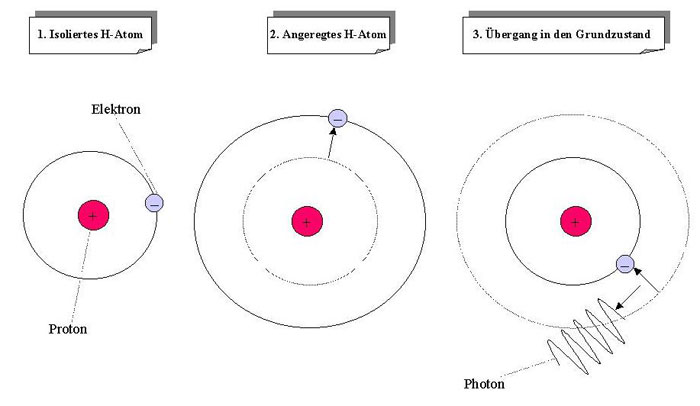
\includegraphics[width = 5cm]{./pictures/wasserstoffBohr}
		 	
		 	Spektrum Balmer-Serie
		 	
		 	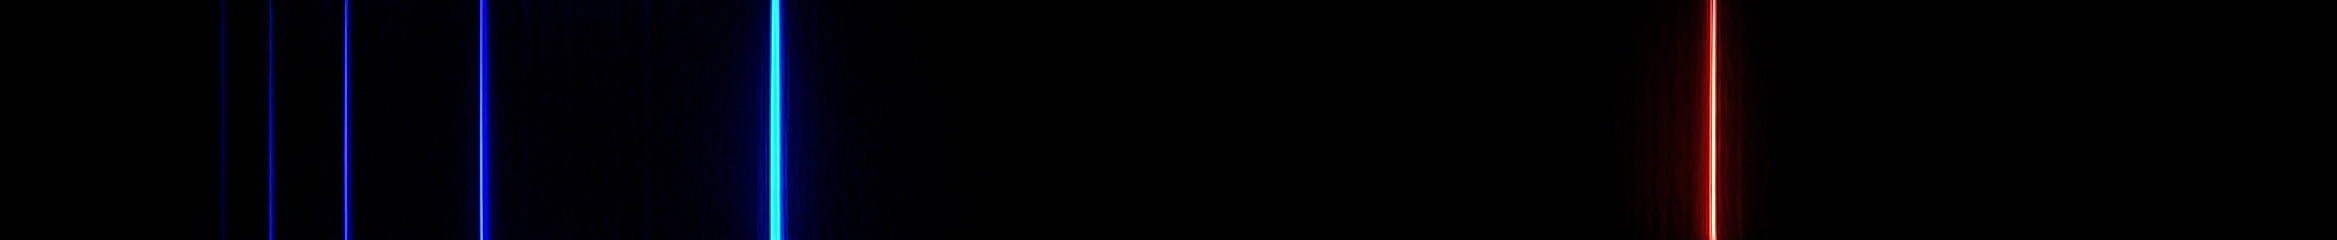
\includegraphics[width = 5cm]{./pictures/wasserstoffSpektrum}
	
	\end{columns}

\end{frame}

\begin{frame}
  \frametitle{Feinstruktur�bergang}
	\begin{columns}
		\column{.5\textwidth}
		\begin{itemize}
		\item[] Betrachtung Spektrum
		\item[] Spin-Bahn Kopplung
		\end{itemize}
		
		\column{.5\textwidth}
		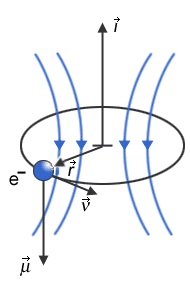
\includegraphics[width = 4cm]{./pictures/feinstrukturelektron}
		
	
		
	\end{columns}
	
\end{frame}

\begin{frame}
	\frametitle{Hyperfeinstruktur�bergang}
	Wechselwirkung zwischen Spin und elektron
	Anwendung St�rungstheorie -> kleine Effekte summieren sich
	Atom haben niedriges niveau -> anregung -> einige werden h�heres Niveau bekommen
	
\end{frame}

\begin{frame}
	\frametitle{Alkalimetalle}
	Abgeschlossene Schalen haben verschwindenden Drehimplus -> nur �usserstes elektron reagiert
	1 Valenzelektron
\end{frame}


%%% Local Variables: 
%%% mode: latex
%%% TeX-master: "../main"
%%% End: 

	
	% 02_Tech; Technischer Aufbau
	\section[Tech]{Technische Betrachtung}
	% 02_analyse

\subsection{Regelkreis}
\begin{frame}
  \frametitle{Technischer Aufbau}

  \begin{figure}
    \centering
    \begin{tikzpicture}
    [node distance=1.3cm]

    \tikzstyle{conn} = [->,shorten >=0.1cm,>=stealth',very thick];

    \only<1>{\tikzstyle{connLamp} = [->,shorten
      >=0.1cm,>=stealth',very thick];}
    \only<2->{\tikzstyle{connLamp} =
      [->,decorate,decoration={snake,amplitude=1.5mm,segment
        length=1.7mm,post length=2.7mm},shorten
      >=0.1cm,>=stealth',very thick,color=red!50!black];}

    \only<-2>{\tikzstyle{connAbsorber} = [->,shorten
      >=0.1cm,>=stealth',very thick];}
    \only<3->{\tikzstyle{connAbsorber} = [->,shorten
      >=0.1cm,>=stealth',line width=1mm];}
    \only<6->{\tikzstyle{connAbsorber} = [->,shorten
      >=0.1cm,>=stealth',semithick];}

    \only<-3>{\tikzstyle{connHfgen} = [->,shorten
      >=0.1cm,>=stealth',very thick];}
    \only<4->{\tikzstyle{connHfgen} =
      [->,decorate,decoration={snake,amplitude=1.5mm,segment
        length=9mm,post length=2.5mm},shorten >=0.1cm,>=stealth',very
      thick]; }

    \only<1>{\tikzstyle{lamp} = [draw,thick,circle,inner sep=1.5mm];}
    \only<2->{\tikzstyle{lamp} = [draw=red!50!black,thick,circle,inner sep=1.5mm,
      fill=red!30];}

    \tikzstyle{absorber} = [draw,thick,circle, inner sep=1.5mm];
    \tikzstyle{vcxo} = [draw,thick, rectangle, inner sep=5mm, align=center];
    \tikzstyle{hfgen} = [draw,thick, rectangle, inner sep=5mm];

    \node[lamp] (lamp) {\ce{^{87}Ru}};
    \only<-4>{\node[absorber] (absorber) [right=of lamp]
    {\(
      \begin{matrix}
        & \downarrow & \uparrow\\
        \uparrow & \downarrow &\\
        & \uparrow & \downarrow\\
        \downarrow & & \uparrow
      \end{matrix}
    \)}; }
    \only<5->{\node[absorber] (absorber) [right=of lamp]
    {\(
      \begin{matrix}
        & \uparrow & \uparrow\\
        \uparrow & \uparrow &\\
        & \uparrow & \uparrow\\
        \uparrow & & \uparrow
      \end{matrix}
    \)}; }
    \node (diode) [right=of absorber] {};
    \draw[semithick](diode) ++ (0.0,-1.0) to[empty photodiode] ++ (0.0,2.0);
    \node[vcxo] (vcxo) [right=of diode]
    {\SI{20}{\mega\hertz}\\VCXO};
    \node[hfgen] (hfgen) [below=of absorber] {\(\times\)};

    \only<2>{\node[] (note) [left=of hfgen] {\SI{750}{\nano\meter}}; }
    \only<4>{\node[xshift=1cm] (note) [left=of hfgen]
      {\SI{6.8346875}{\giga\hertz}}; }

    % connections
    \draw[connLamp] (lamp.east) -- (absorber.west);
    \draw[connAbsorber, shorten >=0.4cm] (absorber.east) -- (diode.west);
    \draw[conn] (diode.east) ++ (0.3cm,0.0) -- (vcxo.west);
    \draw[conn] (vcxo.south) |- (hfgen.east);
    \draw[connHfgen] (hfgen.north) -- (absorber.south);
  \end{tikzpicture}
 \end{figure}
\end{frame}





%%% Local Variables: 
%%% mode: latex
%%% TeX-master: "../main"
%%% End: 
 
		
	% 04_Schluss/Fragen
	\section[?]{ Schluss/Fragen}
	% 07_schluss

%% Periodic Table addapted from http://www.texample.net/tikz/examples/periodic-table-of-chemical-elements/

\newcommand{\CommonElementTextFormat}[4]
{
	\begin{minipage}{2.2cm}
		\centering
		{\textbf{#1} \hfill #2}%
		\linebreak \linebreak
		{\textbf{#3}}%
		\linebreak \linebreak
		{{#4}}
	\end{minipage}
}

\newcommand{\NaturalElementTextFormat}[4]
{
	\CommonElementTextFormat{#1}{#2}{\Huge {#3}}{#4}
}

% \newcommand{\OutlineText}[1]
% {
%   % Couldn't find a nicer way of doing an outline font with TikZ
%   % other than using pdfliteral 1 Tr
%   %
%   \pdfliteral direct {0.5 w 1 Tr}{#1}%
%   \pdfliteral direct {1 w 0 Tr}%
% }

\newcommand{\SyntheticElementTextFormat}[4]
{
	%  \CommonElementTextFormat{#1}{#2}{\OutlineText{\LARGE #3}}{#4}
	\CommonElementTextFormat{#1}{#2}{\Huge #3}{#4}
}

\subsection{Vergleich Atomuhren}

\begin{frame}
	\frametitle{Vergleich Verschiedener Atomuhren}
	
	\begin{columns}
		\column{.5\textwidth}
		\begin{description}
			\item[1949] Ammoniak
			\item[1952] NBS-1
			\item[1967] \num{9192631770} Caesium-133
			\item<2>[1998] Frequenzkamm
			\item<2>[2014] \num{e-18}
		\end{description}
		
		\column{.5\textwidth}
		\centering
		\begin{tabularx}{\columnwidth}{X r r}
			Quarz         & & \num{e-5}\\
			OCXO          & \SI{10}{\mega\hertz}    & \num{2e-8}\\
			\ce{NH3}      & \SI{23.79}{\giga\hertz} & \num{2e-8}\\
			\ce{^{87}Ru}  & \SI{6.83}{\giga\hertz}  & \num{e-9}\\
			\ce{^{133}Cs} & \SI{9.19}{\giga\hertz}  & \num{e-15}\\
			\ce{^{1}H}    & \SI{1.42}{\giga\hertz}  & \num{5e-16}
		\end{tabularx}
	\end{columns}
	
\end{frame}

\begin{frame}
	\frametitle{Verwendete Elemente}
	
	\begin{figure}
		\centering
		\begin{tikzpicture}[font=\sffamily, scale=0.21, transform shape]
		
		%% Fill Color Styles
		\tikzstyle{ElementFill} = [fill=yellow!15]
		\tikzstyle{AlkaliMetalFill} = [fill=blue!55]
		\tikzstyle{AlkalineEarthMetalFill} = [fill=blue!40]
		\tikzstyle{MetalFill} = [fill=blue!25]
		\tikzstyle{MetalloidFill} = [fill=orange!25]
		\tikzstyle{NonmetalFill} = [fill=green!25]
		\tikzstyle{HalogenFill} = [fill=green!40]
		\tikzstyle{NobleGasFill} = [fill=green!55]
		\tikzstyle{LanthanideActinideFill} = [fill=purple!25]
		\tikzstyle{AtomicClockElecFill} = [fill=yellow!75]
		\tikzstyle{AtomicClockOpticFill} = [fill=red!75]
		
		%% Element Styles
		\tikzstyle{Element} = [draw=black, ElementFill,
		minimum width=2.75cm, minimum height=2.75cm, node distance=2.75cm]
		\tikzstyle{AlkaliMetal} = [Element, AlkaliMetalFill]
		\tikzstyle{AlkalineEarthMetal} = [Element, AlkalineEarthMetalFill]
		\tikzstyle{Metal} = [Element, MetalFill]
		\tikzstyle{Metalloid} = [Element, MetalloidFill]
		\tikzstyle{Nonmetal} = [Element, NonmetalFill]
		\tikzstyle{Halogen} = [Element, HalogenFill]
		\tikzstyle{NobleGas} = [Element, NobleGasFill]
		\tikzstyle{LanthanideActinide} = [Element, LanthanideActinideFill]
		\tikzstyle{AtomicClockElec} = [Element, AtomicClockElecFill]
		\tikzstyle{AtomicClockOptic} = [Element, AtomicClockOpticFill]
		\tikzstyle{PeriodLabel} = [font={\sffamily\LARGE}, node distance=2.0cm]
		\tikzstyle{GroupLabel} = [font={\sffamily\LARGE}, minimum width=2.75cm, node distance=2.0cm]
		\tikzstyle{TitleLabel} = [font={\sffamily\Huge\bfseries}]
		
		%% Group 1 - IA
		\only<1>{  \node[name=H, Element] {\NaturalElementTextFormat{1}{1.0079}{H}{Hydrogen}};}
		\only<2->{  \node[name=H, AtomicClockElec] {\NaturalElementTextFormat{1}{1.0079}{H}{Hydrogen}};}
		\node[name=Li, below of=H, AlkaliMetal] {\NaturalElementTextFormat{3}{6.941}{Li}{Lithium}};
		\node[name=Na, below of=Li, AlkaliMetal] {\NaturalElementTextFormat{11}{22.990}{Na}{Sodium}};
		\node[name=K, below of=Na, AlkaliMetal] {\NaturalElementTextFormat{19}{39.098}{K}{Potassium}};
		\only<1>{  \node[name=Rb, below of=K, AlkaliMetal] {\NaturalElementTextFormat{37}{85.468}{Rb}{Rubidium}};}
		\only<2->{  \node[name=Rb, below of=K, AtomicClockElec] {\NaturalElementTextFormat{37}{85.468}{Rb}{Rubidium}};}
		\only<1>{  \node[name=Cs, below of=Rb, AlkaliMetal] {\NaturalElementTextFormat{55}{132.91}{Cs}{Caesium}};}
		\only<2->{  \node[name=Cs, below of=Rb, AtomicClockElec] {\NaturalElementTextFormat{55}{132.91}{Cs}{Caesium}};}
		\node[name=Fr, below of=Cs, AlkaliMetal] {\NaturalElementTextFormat{87}{223}{Fr}{Francium}};
		
		%% Group 2 - IIA
		\only<-2>{  \node[name=Be, right of=Li, AlkalineEarthMetal] {\NaturalElementTextFormat{4}{9.0122}{Be}{Beryllium}};}
		\only<3->{  \node[name=Be, right of=Li, AtomicClockOptic] {\NaturalElementTextFormat{4}{9.0122}{Be}{Beryllium}};}
		\only<-2>{  \node[name=Mg, below of=Be, AlkalineEarthMetal] {\NaturalElementTextFormat{12}{24.305}{Mg}{Magnesium}};}
		\only<3->{  \node[name=Mg, below of=Be, AtomicClockOptic] {\NaturalElementTextFormat{12}{24.305}{Mg}{Magnesium}};}
		\only<-2>{  \node[name=Ca, below of=Mg, AlkalineEarthMetal] {\NaturalElementTextFormat{20}{40.078}{Ca}{Calcium}};}
		\only<3->{  \node[name=Ca, below of=Mg, AtomicClockOptic] {\NaturalElementTextFormat{20}{40.078}{Ca}{Calcium}};}
		\only<-2>{  \node[name=Sr, below of=Ca, AlkalineEarthMetal] {\NaturalElementTextFormat{38}{87.62}{Sr}{Strontium}};}
		\only<3->{  \node[name=Sr, below of=Ca, AtomicClockOptic] {\NaturalElementTextFormat{38}{87.62}{Sr}{Strontium}};}
		\node[name=Ba, below of=Sr, AlkalineEarthMetal] {\NaturalElementTextFormat{56}{137.33}{Ba}{Barium}};
		\node[name=Ra, below of=Ba, AlkalineEarthMetal] {\NaturalElementTextFormat{88}{226}{Ra}{Radium}};
		
		%% Group 3 - IIIB
		\node[name=Sc, right of=Ca, Metal] {\NaturalElementTextFormat{21}{44.956}{Sc}{Scandium}};
		\node[name=Y, below of=Sc, Metal] {\NaturalElementTextFormat{39}{88.906}{Y}{Yttrium}};
		\node[name=LaLu, below of=Y, LanthanideActinide] {\NaturalElementTextFormat{57-71}{}{La-}{Lanthanide}};
		\node[name=AcLr, below of=LaLu, LanthanideActinide] {\NaturalElementTextFormat{89-103}{}{Ac-}{Actinide}};
		% \node[name=LaLu, below of=Y, LanthanideActinide] {\NaturalElementTextFormat{57-71}{}{La-Lu}{Lanthanide}};
		% \node[name=AcLr, below of=LaLu, LanthanideActinide] {\NaturalElementTextFormat{89-103}{}{Ac-Lr}{Actinide}};
		
		%% Group 4 - IVB
		\node[name=Ti, right of=Sc, Metal] {\NaturalElementTextFormat{22}{47.867}{Ti}{Titanium}};
		\node[name=Zr, below of=Ti, Metal] {\NaturalElementTextFormat{40}{91.224}{Zr}{Zirconium}};
		\node[name=Hf, below of=Zr, Metal] {\NaturalElementTextFormat{72}{178.49}{Hf}{Halfnium}};
		\node[name=Rf, below of=Hf, Metal] {\SyntheticElementTextFormat{104}{261}{Rf}{Rutherfordium}};
		
		%% Group 5 - VB
		\node[name=V, right of=Ti, Metal] {\NaturalElementTextFormat{23}{50.942}{V}{Vanadium}};
		\node[name=Nb, below of=V, Metal] {\NaturalElementTextFormat{41}{92.906}{Nb}{Niobium}};
		\node[name=Ta, below of=Nb, Metal] {\NaturalElementTextFormat{73}{180.95}{Ta}{Tantalum}};
		\node[name=Db, below of=Ta, Metal] {\SyntheticElementTextFormat{105}{262}{Db}{Dubnium}};
		
		%% Group 6 - VIB
		\node[name=Cr, right of=V, Metal] {\NaturalElementTextFormat{24}{51.996}{Cr}{Chromium}};
		\node[name=Mo, below of=Cr, Metal] {\NaturalElementTextFormat{42}{95.94}{Mo}{Molybdenum}};
		\node[name=W, below of=Mo, Metal] {\NaturalElementTextFormat{74}{183.84}{W}{Tungsten}};
		\node[name=Sg, below of=W, Metal] {\SyntheticElementTextFormat{106}{266}{Sg}{Seaborgium}};
		
		%% Group 7 - VIIB
		\node[name=Mn, right of=Cr, Metal] {\NaturalElementTextFormat{25}{54.938}{Mn}{Manganese}};
		\node[name=Tc, below of=Mn, Metal] {\NaturalElementTextFormat{43}{96}{Tc}{Technetium}};
		\node[name=Re, below of=Tc, Metal] {\NaturalElementTextFormat{75}{186.21}{Re}{Rhenium}};
		\node[name=Bh, below of=Re, Metal] {\SyntheticElementTextFormat{107}{264}{Bh}{Bohrium}};
		
		%% Group 8 - VIIIB
		\node[name=Fe, right of=Mn, Metal] {\NaturalElementTextFormat{26}{55.845}{Fe}{Iron}};
		\node[name=Ru, below of=Fe, Metal] {\NaturalElementTextFormat{44}{101.07}{Ru}{Ruthenium}};
		\node[name=Os, below of=Ru, Metal] {\NaturalElementTextFormat{76}{190.23}{Os}{Osmium}};
		\node[name=Hs, below of=Os, Metal] {\SyntheticElementTextFormat{108}{277}{Hs}{Hassium}};
		
		%% Group 9 - VIIIB
		\node[name=Co, right of=Fe, Metal] {\NaturalElementTextFormat{27}{58.933}{Co}{Cobalt}};
		\node[name=Rh, below of=Co, Metal] {\NaturalElementTextFormat{45}{102.91}{Rh}{Rhodium}};
		\node[name=Ir, below of=Rh, Metal] {\NaturalElementTextFormat{77}{192.22}{Ir}{Iridium}};
		\node[name=Mt, below of=Ir, Metal] {\SyntheticElementTextFormat{109}{268}{Mt}{Meitnerium}};
		
		%% Group 10 - VIIIB
		\node[name=Ni, right of=Co, Metal] {\NaturalElementTextFormat{28}{58.693}{Ni}{Nickel}};
		\node[name=Pd, below of=Ni, Metal] {\NaturalElementTextFormat{46}{106.42}{Pd}{Palladium}};
		\node[name=Pt, below of=Pd, Metal] {\NaturalElementTextFormat{78}{195.08}{Pt}{Platinum}};
		\node[name=Ds, below of=Pt, Metal] {\SyntheticElementTextFormat{110}{281}{Ds}{Darmstadtium}};
		
		%% Group 11 - IB
		\node[name=Cu, right of=Ni, Metal] {\NaturalElementTextFormat{29}{63.546}{Cu}{Copper}};
		\node[name=Ag, below of=Cu, Metal] {\NaturalElementTextFormat{47}{107.87}{Ag}{Silver}};
		\node[name=Au, below of=Ag, Metal] {\NaturalElementTextFormat{79}{196.97}{Au}{Gold}};
		\node[name=Rg, below of=Au, Metal] {\SyntheticElementTextFormat{111}{280}{Rg}{Roentgenium}};
		
		%% Group 12 - IIB
		\node[name=Zn, right of=Cu, Metal] {\NaturalElementTextFormat{30}{65.39}{Zn}{Zinc}};
		\node[name=Cd, below of=Zn, Metal] {\NaturalElementTextFormat{48}{112.41}{Cd}{Cadmium}};
		\only<-2>{  \node[name=Hg, below of=Cd, Metal] {\NaturalElementTextFormat{80}{200.59}{Hg}{Mercury}};}
		\only<3->{  \node[name=Hg, below of=Cd, AtomicClockOptic] {\NaturalElementTextFormat{80}{200.59}{Hg}{Mercury}};}
		\node[name=Uub, below of=Hg, Metal] {\SyntheticElementTextFormat{112}{285}{Uub}{Ununbium}};
		
		%% Group 13 - IIIA
		\node[name=Ga, right of=Zn, Metal] {\NaturalElementTextFormat{31}{69.723}{Ga}{Gallium}};
		\only<-2>{  \node[name=Al, above of=Ga, Metal] {\NaturalElementTextFormat{13}{26.982}{Al}{Aluminium}};}
		\only<3->{  \node[name=Al, above of=Ga, AtomicClockOptic] {\NaturalElementTextFormat{13}{26.982}{Al}{Aluminium}};}
		\node[name=B, above of=Al, Metalloid] {\NaturalElementTextFormat{5}{10.811}{B}{Boron}};
		\only<-2>{  \node[name=In, below of=Ga, Metal] {\NaturalElementTextFormat{49}{114.82}{In}{Indium}};}
		\only<3->{  \node[name=In, below of=Ga, AtomicClockOptic] {\NaturalElementTextFormat{49}{114.82}{In}{Indium}};}
		\node[name=Tl, below of=In, Metal] {\NaturalElementTextFormat{81}{204.38}{Tl}{Thallium}};
		\node[name=Uut, below of=Tl, Metal] {\SyntheticElementTextFormat{113}{284}{Uut}{Ununtrium}};
		
		%% Group 14 - IVA
		\node[name=C, right of=B, Nonmetal] {\NaturalElementTextFormat{6}{12.011}{C}{Carbon}};
		\node[name=Si, below of=C, Metalloid] {\NaturalElementTextFormat{14}{28.086}{Si}{Silicon}};
		\node[name=Ge, below of=Si, Metalloid] {\NaturalElementTextFormat{32}{72.64}{Ge}{Germanium}};
		\node[name=Sn, below of=Ge, Metal] {\NaturalElementTextFormat{50}{118.71}{Sn}{Tin}};
		\node[name=Pb, below of=Sn, Metal] {\NaturalElementTextFormat{82}{207.2}{Pb}{Lead}};
		\node[name=Uuq, below of=Pb, Metal] {\SyntheticElementTextFormat{114}{289}{Uuq}{Ununquadium}};
		
		%% Group 15 - VA
		\node[name=N, right of=C, Nonmetal] {\NaturalElementTextFormat{7}{14.007}{N}{Nitrogen}};
		\node[name=P, below of=N, Nonmetal] {\NaturalElementTextFormat{15}{30.974}{P}{Phosphorus}};
		\node[name=As, below of=P, Metalloid] {\NaturalElementTextFormat{33}{74.922}{As}{Arsenic}};
		\node[name=Sb, below of=As, Metalloid] {\NaturalElementTextFormat{51}{121.76}{Sb}{Antimony}};
		\node[name=Bi, below of=Sb, Metal] {\NaturalElementTextFormat{83}{208.98}{Bi}{Bismuth}};
		\node[name=Uup, below of=Bi, Metal] {\SyntheticElementTextFormat{115}{288}{Uup}{Ununpentium}};
		
		%% Group 16 - VIA
		\node[name=O, right of=N, Nonmetal] {\NaturalElementTextFormat{8}{15.999}{O}{Oxygen}};
		\node[name=S, below of=O, Nonmetal] {\NaturalElementTextFormat{16}{32.065}{S}{Sulphur}};
		\node[name=Se, below of=S, Nonmetal] {\NaturalElementTextFormat{34}{78.96}{Se}{Selenium}};
		\node[name=Te, below of=Se, Metalloid] {\NaturalElementTextFormat{52}{127.6}{Te}{Tellurium}};
		\node[name=Po, below of=Te, Metalloid] {\NaturalElementTextFormat{84}{209}{Po}{Polonium}};
		\node[name=Uuh, below of=Po, Metal] {\SyntheticElementTextFormat{116}{293}{Uuh}{Ununhexium}};
		
		%% Group 17 - VIIA
		\node[name=F, right of=O, Halogen] {\NaturalElementTextFormat{9}{18.998}{F}{Flourine}};
		\node[name=Cl, below of=F, Halogen] {\NaturalElementTextFormat{17}{35.453}{Cl}{Chlorine}};
		\node[name=Br, below of=Cl, Halogen] {\NaturalElementTextFormat{35}{79.904}{Br}{Bromine}};
		\node[name=I, below of=Br, Halogen] {\NaturalElementTextFormat{53}{126.9}{I}{Iodine}};
		\node[name=At, below of=I, Halogen] {\NaturalElementTextFormat{85}{210}{At}{Astatine}};
		\node[name=Uus, below of=At, Element] {\SyntheticElementTextFormat{117}{292}{Uus}{Ununseptium}}; 
		
		%% Group 18 - VIIIA
		\node[name=Ne, right of=F, NobleGas] {\NaturalElementTextFormat{10}{20.180}{Ne}{Neon}};
		\node[name=He, above of=Ne, NobleGas] {\NaturalElementTextFormat{2}{4.0025}{He}{Helium}};
		\node[name=Ar, below of=Ne, NobleGas] {\NaturalElementTextFormat{18}{39.948}{Ar}{Argon}};
		\node[name=Kr, below of=Ar, NobleGas] {\NaturalElementTextFormat{36}{83.8}{Kr}{Krypton}};
		\node[name=Xe, below of=Kr, NobleGas] {\NaturalElementTextFormat{54}{131.29}{Xe}{Xenon}};
		\node[name=Rn, below of=Xe, NobleGas] {\NaturalElementTextFormat{86}{222}{Rn}{Radon}};
		\node[name=Uuo, below of=Rn, Nonmetal] {\SyntheticElementTextFormat{118}{294}{Uuo}{Ununoctium}}; 
		
		%% Period
		\node[name=Period1, left of=H, PeriodLabel] {1};
		\node[name=Period2, left of=Li, PeriodLabel] {2};
		\node[name=Period3, left of=Na, PeriodLabel] {3}; 
		\node[name=Period4, left of=K, PeriodLabel] {4}; 
		\node[name=Period5, left of=Rb, PeriodLabel] {5};
		\node[name=Period6, left of=Cs, PeriodLabel] {6};
		\node[name=Period7, left of=Fr, PeriodLabel] {7};
		
		%% Group
		\node[name=Group1, above of=H, GroupLabel] {1 \hfill IA};
		\node[name=Group2, above of=Be, GroupLabel] {2 \hfill IIA};
		\node[name=Group3, above of=Sc, GroupLabel] {3 \hfill IIIA};
		\node[name=Group4, above of=Ti, GroupLabel] {4 \hfill IVB};
		\node[name=Group5, above of=V, GroupLabel] {5 \hfill VB};
		\node[name=Group6, above of=Cr, GroupLabel] {6 \hfill VIB};
		\node[name=Group7, above of=Mn, GroupLabel] {7 \hfill VIIB};
		\node[name=Group8, above of=Fe, GroupLabel] {8 \hfill VIIIB};
		\node[name=Group9, above of=Co, GroupLabel] {9 \hfill VIIIB};
		\node[name=Group10, above of=Ni, GroupLabel] {10 \hfill VIIIB};
		\node[name=Group11, above of=Cu, GroupLabel] {11 \hfill IB};
		\node[name=Group12, above of=Zn, GroupLabel] {12 \hfill IIB};
		\node[name=Group13, above of=B, GroupLabel] {13 \hfill IIIA};
		\node[name=Group14, above of=C, GroupLabel] {14 \hfill IVA};
		\node[name=Group15, above of=N, GroupLabel] {15 \hfill VA};
		\node[name=Group16, above of=O, GroupLabel] {16 \hfill VIA};
		\node[name=Group17, above of=F, GroupLabel] {17 \hfill VIIA};
		\node[name=Group18, above of=He, GroupLabel] {18 \hfill VIIIA};
		
		%% Lanthanide
		\node[name=La, below of=Rf, LanthanideActinide, yshift=-1cm] {\NaturalElementTextFormat{57}{138.91}{La}{Lanthanum}};
		\node[name=Ce, right of=La, LanthanideActinide] {\NaturalElementTextFormat{58}{140.12}{Ce}{Cerium}};
		\node[name=Pr, right of=Ce, LanthanideActinide] {\NaturalElementTextFormat{59}{140.91}{Pr}{Praseodymium}};
		\node[name=Nd, right of=Pr, LanthanideActinide] {\NaturalElementTextFormat{60}{144.24}{Nd}{Neodymium}};
		\node[name=Pm, right of=Nd, LanthanideActinide] {\NaturalElementTextFormat{61}{145}{Pm}{Promethium}};
		\node[name=Sm, right of=Pm, LanthanideActinide] {\NaturalElementTextFormat{62}{150.36}{Sm}{Samarium}};
		\node[name=Eu, right of=Sm, LanthanideActinide] {\NaturalElementTextFormat{63}{151.96}{Eu}{Europium}};
		\node[name=Gd, right of=Eu, LanthanideActinide] {\NaturalElementTextFormat{64}{157.25}{Gd}{Gadolinium}};
		\node[name=Tb, right of=Gd, LanthanideActinide] {\NaturalElementTextFormat{65}{158.93}{Tb}{Terbium}};
		\node[name=Dy, right of=Tb, LanthanideActinide] {\NaturalElementTextFormat{66}{162.50}{Dy}{Dysprosium}};
		\node[name=Ho, right of=Dy, LanthanideActinide] {\NaturalElementTextFormat{67}{164.93}{Ho}{Holmium}};
		\node[name=Er, right of=Ho, LanthanideActinide] {\NaturalElementTextFormat{68}{167.26}{Er}{Erbium}};
		\node[name=Tm, right of=Er, LanthanideActinide] {\NaturalElementTextFormat{69}{168.93}{Tm}{Thulium}};
		\only<-2>{  \node[name=Yb, right of=Tm, LanthanideActinide] {\NaturalElementTextFormat{70}{173.04}{Yb}{Ytterbium}};}
		\only<3->{  \node[name=Yb, right of=Tm, AtomicClockOptic] {\NaturalElementTextFormat{70}{173.04}{Yb}{Ytterbium}};}
		\node[name=Lu, right of=Yb, LanthanideActinide] {\NaturalElementTextFormat{71}{174.97}{Lu}{Lutetium}};
		
		%% Actinide
		\node[name=Ac, below of=La, LanthanideActinide, yshift=-1cm] {\NaturalElementTextFormat{89}{227}{Ac}{Actinium}};
		\node[name=Th, right of=Ac, LanthanideActinide] {\NaturalElementTextFormat{90}{232.04}{Th}{Thorium}};
		\node[name=Pa, right of=Th, LanthanideActinide] {\NaturalElementTextFormat{91}{231.04}{Pa}{Protactinium}};
		\node[name=U, right of=Pa, LanthanideActinide] {\NaturalElementTextFormat{92}{238.03}{U}{Uranium}};
		\node[name=Np, right of=U, LanthanideActinide] {\SyntheticElementTextFormat{93}{237}{Np}{Neptunium}};
		\node[name=Pu, right of=Np, LanthanideActinide] {\SyntheticElementTextFormat{94}{244}{Pu}{Plutonium}};
		\node[name=Am, right of=Pu, LanthanideActinide] {\SyntheticElementTextFormat{95}{243}{Am}{Americium}};
		\node[name=Cm, right of=Am, LanthanideActinide] {\SyntheticElementTextFormat{96}{247}{Cm}{Curium}};
		\node[name=Bk, right of=Cm, LanthanideActinide] {\SyntheticElementTextFormat{97}{247}{Bk}{Berkelium}};
		\node[name=Cf, right of=Bk, LanthanideActinide] {\SyntheticElementTextFormat{98}{251}{Cf}{Californium}};
		\node[name=Es, right of=Cf, LanthanideActinide] {\SyntheticElementTextFormat{99}{252}{Es}{Einsteinium}};
		\node[name=Fm, right of=Es, LanthanideActinide] {\SyntheticElementTextFormat{100}{257}{Fm}{Fermium}};
		\node[name=Md, right of=Fm, LanthanideActinide] {\SyntheticElementTextFormat{101}{258}{Md}{Mendelevium}};
		\node[name=No, right of=Md, LanthanideActinide] {\SyntheticElementTextFormat{102}{259}{No}{Nobelium}};
		\node[name=Lr, right of=No, LanthanideActinide] {\SyntheticElementTextFormat{103}{262}{Lr}{Lawrencium}};
		
		%% Draw dotted lines connecting Lanthanide breakout to main table
		\draw (LaLu.north west) edge[dotted] (La.north west)
		(LaLu.north east) edge[dotted] (Lu.north east)
		(LaLu.south west) edge[dotted] (La.south west)
		(LaLu.south east) edge[dotted] (Lu.south east);
		%% Draw dotted lines connecting Actinide breakout to main table
		\draw (AcLr.north west) edge[dotted] (Ac.north west)
		(AcLr.north east) edge[dotted] (Lr.north east)
		(AcLr.south west) edge[dotted] (Ac.south west)
		(AcLr.south east) edge[dotted] (Lr.south east);
		
		% %% Legend
		%   \draw[black, AlkaliMetalFill] ($(La.north -| Fr.west) + (1em,-0.0em)$)
		%     rectangle +(1em, 1em) node[right, yshift=-1ex]{Alkali Metal};
		%   \draw[black, AlkalineEarthMetalFill] ($(La.north -| Fr.west) + (1em,-1.5em)$)
		%     rectangle +(1em, 1em) node[right, yshift=-1ex]{Alkaline Earth Metal};
		%   \draw[black, MetalFill] ($(La.north -| Fr.west) + (1em,-3.0em)$)
		%     rectangle +(1em, 1em) node[right, yshift=-1ex]{Metal};
		%   \draw[black, MetalloidFill] ($(La.north -| Fr.west) + (1em,-4.5em)$)
		%     rectangle +(1em, 1em) node[right, yshift=-1ex]{Metalloid};
		%   \draw[black, NonmetalFill] ($(La.north -| Fr.west) + (1em,-6.0em)$)
		%     rectangle +(1em, 1em) node[right, yshift=-1ex]{Non-metal};
		%   \draw[black, HalogenFill] ($(La.north -| Fr.west) + (1em,-7.5em)$)
		%     rectangle +(1em, 1em) node[right, yshift=-1ex]{Halogen};
		%   \draw[black, NobleGasFill] ($(La.north -| Fr.west) + (1em,-9.0em)$)
		%     rectangle +(1em, 1em) node[right, yshift=-1ex]{Noble Gas};
		%   \draw[black, LanthanideActinideFill] ($(La.north -| Fr.west) + (1em,-10.5em)$)
		%     rectangle +(1em, 1em) node[right, yshift=-1ex]{Lanthanide/Actinide};
		
		%   \node at ($(La.north -| Fr.west) + (5em,-15em)$) [name=elementLegend, Element, fill=white]
		%     {\NaturalElementTextFormat{Z}{mass}{Symbol}{Name}};
		%   \node[Element, fill=white, right of=elementLegend, xshift=1em]
		%     {\SyntheticElementTextFormat{}{}{man-made}{}} ;
		
		% %% Diagram Title
		%   \node at (H.west -| Fe.north) [name=diagramTitle, TitleLabel]
		%     {(Mendeleev's) Periodic Table of Chemical Elements via Ti\emph{k}Z};
		
		\end{tikzpicture}
	\end{figure}
	
	
\end{frame}

\subsection{Schluss}

\begin{frame}
  \frametitle{Schluss}

\end{frame}

\subsection{Fragen}
\begin{frame}
  \frametitle{Fragen}
\end{frame}



%%% Local Variables: 
%%% mode: latex
%%% TeX-master: "../main"
%%% End: 

	
	%%% END DOCUMENT
\end{document}